\documentclass{report}

\usepackage{graphicx} 
\usepackage[export]{adjustbox}
\usepackage{amsmath}
\usepackage{hyperref}
\usepackage[utf8]{inputenc}
\usepackage{booktabs}
\usepackage{caption}
\usepackage{enumitem}

\title{Research Project Proposal}
\author{Iván Peñate Gómez}
\date{\today}

\begin{document}

\maketitle

\chapter*{Research Proposal: A JANI-Exporting Editor for 3D Grid Worlds}
\addcontentsline{toc}{chapter}{10-Week Research Proposal: A JANI-Exporting Editor for 3D Grid Worlds}

\section*{Project Overview}
\addcontentsline{toc}{section}{Project Overview}

This research aims to develop a graphical editor for 3D grid-world environments, export them to the JANI quantitative model interchange format, and perform comparative verification across multiple model checkers (initially Storm, PRISM and Modest Toolset). The project bridges graphical environment design with formal verification, enabling systematic benchmarking of model checkers on a common set of grid-world problems.

\section*{Core Research Questions}
\addcontentsline{toc}{section}{Core Research Questions}

\begin{enumerate}
    \item How can a 3D grid world with heterogeneous elements (agents, walls, elevators, targets, objects) be faithfully encoded in JANI?
    \item What translation algorithms are required to map graphical grid-world specifications to valid JANI models?
    \item How do different model checkers (Storm vs. PRISM vs Modest Toolset) compare in performance and property verification on identical JANI-exported grid-world problems?
    \item Can the editor generate optimal policies that are consistent across model checkers?
\end{enumerate}

\section*{Deliverables}
\addcontentsline{toc}{section}{Deliverables}

\begin{itemize}
    \item Functional 3D grid-world editor (web-based or desktop)
    \item JANI export engine
    \item Integration with Storm, PRISM and Modest Toolset model checkers
    \item Benchmark suite of grid-world configurations with known properties
    \item Comparative performance analysis report
    \item Open-source repository with documentation
\end{itemize}

\section*{10-Week Schedule}

\begin{figure}[h]
\centering
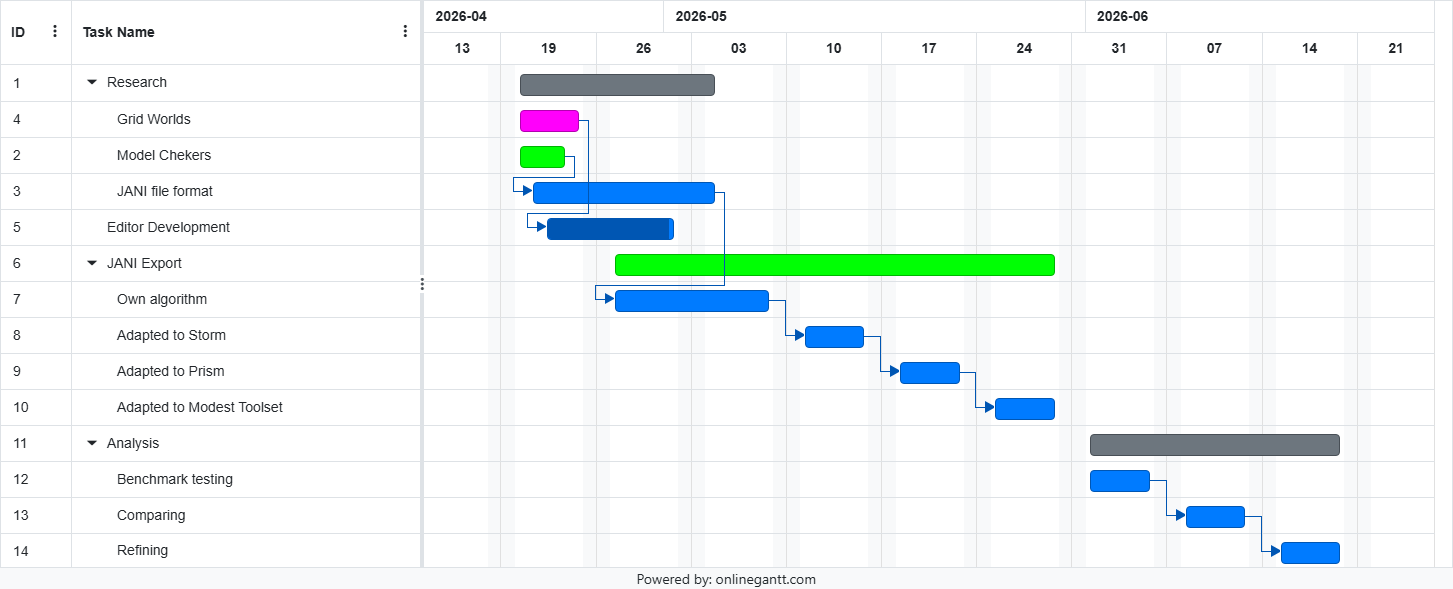
\includegraphics[width=\textwidth]{Online Gantt 20260423.png}
\caption{Gantt Chart}
\label{fig:yourlabel}
\end{figure}

\addcontentsline{toc}{section}{10-Week Schedule}

\begin{table}[h]
\centering
\caption{Weekly breakdown of research activities}
\label{tab:schedule}
\begin{tabular}{|p{1.5cm}|p{11cm}|}
\hline
\textbf{Week} & \textbf{Activities} \\ \hline
1 & \textbf{Literature \and requirements gathering} \\
    & - Understand the JANI file format \\
    & - Study Storm, PRISM and Modest Toolset Checking capabilities \\
    & - Define complete grid-world elements 
    \\ \hline
2 & \textbf{Grid-world editor prototype} \\
    & - Implement basic 3D grid rendering \\
    & - Create cell-type selection interface (wall, agent, target, elevator, object) \\
    & - Implement save/load functionality for world definitions \\
    & \textbf{Core translation algorithm design} \\
    & - Design mapping from grid coordinates to JANI variables \\
    & - Define automaton structure for agents\\
    & - Implement guard generation for movement constraints (walls, bounds) \\
    & - Handle elevator one-way transitions \\
    \hline
3-4 & \textbf{JANI export engine} \\
    & - Generate valid JANI \\
    & - Include variable declarations, automata, edges \\
    & - Export simple test worlds \\ \hline
5 & \textbf{Storm integration} \\
    & - Research on Specifications of Storm \\
    & - Adapt JANI export for the optimality of Storm \\
    & - Visualize output of Storm in the Editor for every world \\ \hline
6 & \textbf{Prism integration} \\
    & - Research on Specifications of Prism \\
    & - Adapt JANI export for the optimality of Prism \\
    & - Visualize output of Prism in the Editor for every world \\ \hline
7 & \textbf{Modest Toolset integration} \\
    & - Research on Specifications of Modest Toolset \\
    & - Adapt JANI export for the optimality of Modest Toolset \\
    & - Visualize output of Modest Toolset in the Editor for every world \\ \hline
8 & \textbf{Benchmark tests development} \\
    & - Create 10--15 diverse grid-world configurations \\
    & - Varying sizes: 3x3x2 to 10x10x3 \\
    & - Varying complexity: obstacles, multi-agent, elevator chains  \\ \hline
9 & \textbf{Comparative analysis} \\
    & - Run benchmark test on Storm, PRISM and Modest Toolset \\
    & - Measure: verification time, memory usage, policy optimality \\
    & - Identify discrepancies and edge cases \\
    & - Write on the report \\ \hline
10 & \textbf{Refinement \and final deliverables} \\
    & - Bug fixes and performance optimisation \\
    & - Complete user documentation \\
    & - Prepare final report and presentation \\
    & - Package repository for open-source release \\ \hline
\end{tabular}
\end{table}

\section*{Technical Architecture}
\addcontentsline{toc}{section}{Technical Architecture}

The system follows a linear pipeline from graphical design to verification results:

\begin{enumerate}
    \item \textbf{3D Grid Editor (Python)}: The user constructs a grid world by placing walls, agents, elevators, targets, and objects in a 3D coordinate system. The editor stores the world as an internal Python data structure (a 3D array of cell types with associated properties).
    
    \item \textbf{JANI Export Engine}: A translation algorithm converts the internal grid representation into a valid JANI file. Each grid cell maps to JANI variables and transitions: walls block movement, elevators create instantaneous floor changes, and targets are encoded with a reward system. Movement actions (north, south, east, west, up, down) become JANI edges with appropriate guards based on agent position.
    
    \item \textbf{Model Checker Integration}: The editor invokes three model checkers (Storm, PRISM, Modest Toolset) as external processes on the generated JANI file. Each checker computes an optimal policy for a user-specified property (e.g., ``reach the target in minimal expected steps''). The editor parses and displays the results: verification time, memory usage, and policy outcome.
    
    \item \textbf{Visualisation Layer}: Results are shown as comparison tables and charts within the editor interface, highlighting performance differences across checkers.
\end{enumerate}

\subsection*{Data Flow Summary}

\begin{center}
User input $\rightarrow$ World state $\rightarrow$ JANI file $\rightarrow$ Results
\end{center}

\section*{Success Criteria}
\addcontentsline{toc}{section}{Success Criteria}

\begin{enumerate}
    \item Editor successfully exports a 3x3x3 grid world to valid JANI
    \item Both Storm, PRISM and Modest Toolset produce valid results for a grid world.
    \item At least 10 benchmark configurations with documented performance metrics
    \item The tool produces a verifiable optimal policy for reachability problems
    \item Complete documentation enabling others to extend the editor
\end{enumerate}

\section*{Required Resources}
\addcontentsline{toc}{section}{Required Resources}

\begin{itemize}
    \item Storm installation (\url{https://www.stormchecker.org})
    \item PRISM installation (\url{https://www.prismmodelchecker.org})
    \item Modest Toolset
    \item Python
\end{itemize}

\section*{Resources Used}

The following online resources provide specifications, documentation, and tool access for JANI and related verification tools:

\begin{itemize}
    \item JANI Specification (Official): \href{https://jani-spec.org/}{jani-spec.org}, Overview of the JANI format, tool support, and model libraries.
    
    \item JANI Specification Document (Google Docs): \href{https://docs.google.com/document/d/1BDQIzPBtscxJFFlDUEPIo8ivKHgXT8_X6hz5quq7jK0/edit}{Working specification}, Detailed technical reference for JANI syntax and semantics.
    
    \item Model Checking (Wikipedia): \href{https://en.wikipedia.org/wiki/Model_checking}{Model checking}, General background on formal verification techniques.
    
    \item Modest Toolset: \href{https://www.modestchecker.net/}{modestchecker.net}, Homepage of the Modest Toolset, which supports JANI import/export and verification.
    
    \item Storm Checker: \href{https://www.stormchecker.org}{stormchecker.org}, High-performance probabilistic model checker with strong JANI support.
    
    \item PRISM Model Checker: \href{https://www.prismmodelchecker.org}{prismmodelchecker.org}, Widely used probabilistic model checker with JANI capabilities.
\end{itemize}

These resources will guide the implementation of the JANI export engine and the integration with model checkers for the grid-world editor.

\section*{Conclusion}
\addcontentsline{toc}{section}{Conclusion}

This 10-week proposal outlines a feasible path from a 3D grid-world editor to comparative model checking via JANI. The schedule allocates two weeks for foundational work (literature + basic editor), four weeks for core JANI translation and tool integration, two weeks for benchmarking, and two weeks for analysis and refinement. The primary contribution will be an open source tool that lowers the barrier to using formal verification on grid-world problems while providing empirical data on model checker performance.

\end{document}